\documentclass[tikz,border=12pt]{standalone}
\usepackage[T1]{fontenc}
\usepackage{mathpazo}
\usepackage{amsmath,amssymb}
\usetikzlibrary{arrows.meta, positioning, calc}

\definecolor{stblue}{HTML}{7B97AD}
\definecolor{rwgold}{HTML}{B8995E}
\definecolor{sage}{HTML}{7A9A7E}
\definecolor{dkbrown}{HTML}{3D3530}
\definecolor{wmgray}{HTML}{7B7067}
\definecolor{cream}{HTML}{F9F6F0}
\definecolor{border}{HTML}{D4C9B8}
\definecolor{terracotta}{HTML}{C47A6A}
\definecolor{lavender}{HTML}{907EA0}

\begin{document}
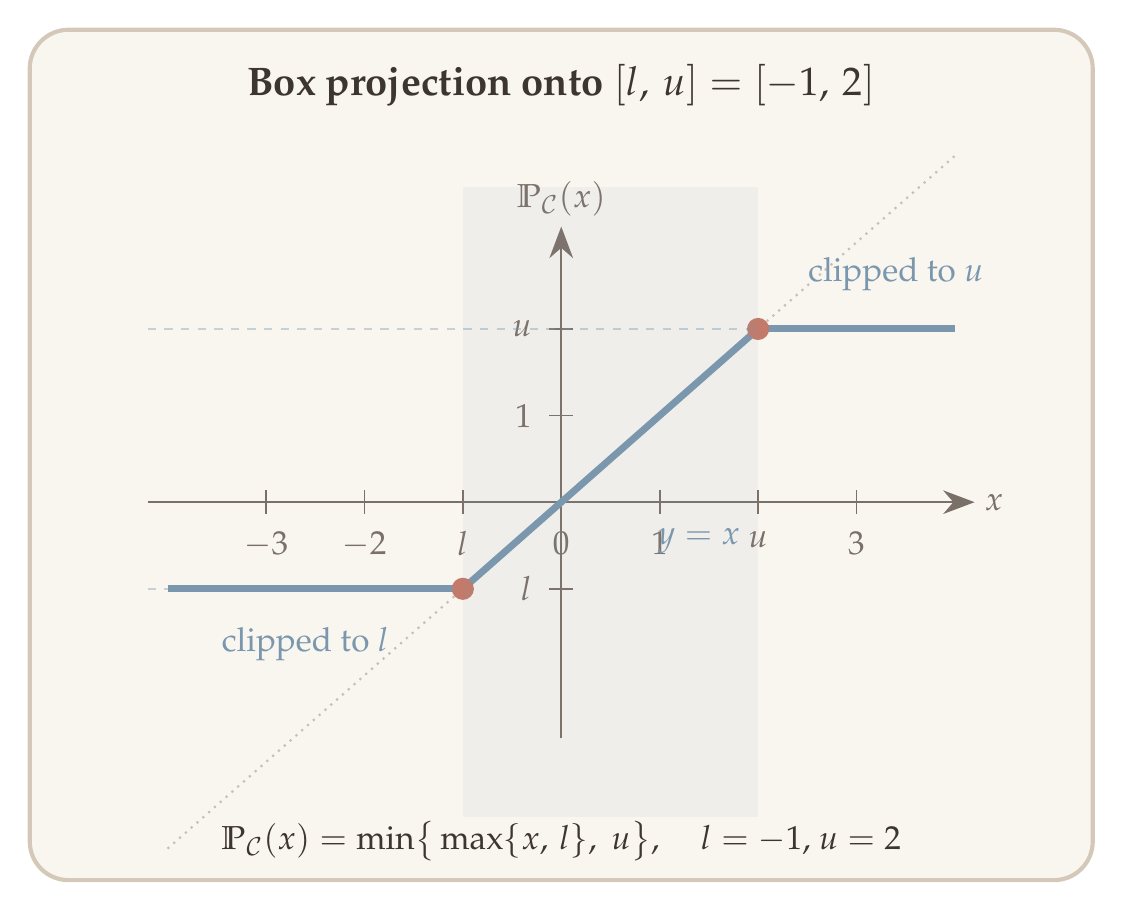
\begin{tikzpicture}[>={Stealth[length=4mm, width=3mm]}]

% Background
\fill[cream, rounded corners=14pt] (-0.5,-0.8) rectangle (13,10);
\draw[border, line width=1.5pt, rounded corners=14pt] (-0.5,-0.8) rectangle (13,10);

% Title
\node[text=dkbrown, font=\Large\bfseries] at (6.25,9.3)
  {Box projection onto $[l,\, u] = [-1,\, 2]$};

% Coordinate mapping:
% x-range: -4 to 4, center at canvas x=6.25
% y-range: -2 to 3, center at canvas y=4.0
% x-scale: 1.25, y-scale: 1.1

% Axes
\draw[wmgray, line width=0.8pt, ->] (1.0,4.0) -- (11.5,4.0)
  node[right, font=\large, text=wmgray] {$x$};
\draw[wmgray, line width=0.8pt, ->] (6.25,1.0) -- (6.25,7.5)
  node[above, font=\large, text=wmgray] {$\mathbb{P}_\mathcal{C}(x)$};

% x -> 6.25 + x*1.25
% y -> 4.0 + y*1.1

% Tick marks x-axis
\draw[wmgray, line width=0.6pt] (6.25,3.85) -- (6.25,4.15);
\node[text=wmgray, font=\large, below] at (6.25,3.75) {$0$};

% l=-1 -> 6.25 + (-1)*1.25 = 5.0
\draw[wmgray, line width=0.6pt] (5.0,3.85) -- (5.0,4.15);
\node[text=wmgray, font=\large, below] at (5.0,3.75) {$l$};

% u=2 -> 6.25 + 2*1.25 = 8.75
\draw[wmgray, line width=0.6pt] (8.75,3.85) -- (8.75,4.15);
\node[text=wmgray, font=\large, below] at (8.75,3.75) {$u$};

\draw[wmgray, line width=0.6pt] (3.75,3.85) -- (3.75,4.15);
\node[text=wmgray, font=\large, below] at (3.75,3.75) {$-2$};
\draw[wmgray, line width=0.6pt] (2.5,3.85) -- (2.5,4.15);
\node[text=wmgray, font=\large, below] at (2.5,3.75) {$-3$};
\draw[wmgray, line width=0.6pt] (7.5,3.85) -- (7.5,4.15);
\node[text=wmgray, font=\large, below] at (7.5,3.75) {$1$};
\draw[wmgray, line width=0.6pt] (10.0,3.85) -- (10.0,4.15);
\node[text=wmgray, font=\large, below] at (10.0,3.75) {$3$};

% Y-axis ticks
% l=-1 -> 4.0 + (-1)*1.1 = 2.9
\draw[wmgray, line width=0.6pt] (6.1,2.9) -- (6.4,2.9);
\node[text=wmgray, font=\large, left] at (6.0,2.9) {$l$};
% u=2 -> 4.0 + 2*1.1 = 6.2
\draw[wmgray, line width=0.6pt] (6.1,6.2) -- (6.4,6.2);
\node[text=wmgray, font=\large, left] at (6.0,6.2) {$u$};
\draw[wmgray, line width=0.6pt] (6.1,5.1) -- (6.4,5.1);
\node[text=wmgray, font=\large, left] at (6.0,5.1) {$1$};

% Identity line (dotted reference)
\draw[wmgray, line width=0.8pt, dotted, opacity=0.4]
  (1.25, {4.0 + (-4)*1.1}) -- (11.25, {4.0 + 4*1.1});

% Box projection function: min(max(x, l), u) with l=-1, u=2
% Three pieces:
% 1) x <= -1: y = -1 -> from x=-4 to x=-1
%    canvas: (1.25, 2.9) to (5.0, 2.9)
\draw[stblue, line width=2.5pt] (1.25, 2.9) -- (5.0, 2.9);

% 2) -1 <= x <= 2: y = x -> from x=-1 to x=2
%    canvas: (5.0, 2.9) to (8.75, 6.2)
\draw[stblue, line width=2.5pt] (5.0, 2.9) -- (8.75, 6.2);

% 3) x >= 2: y = 2 -> from x=2 to x=4
%    canvas: (8.75, 6.2) to (11.25, 6.2)
\draw[stblue, line width=2.5pt] (8.75, 6.2) -- (11.25, 6.2);

% Breakpoint markers
\fill[terracotta] (5.0,2.9) circle (4pt);
\fill[terracotta] (8.75,6.2) circle (4pt);

% Dashed lines showing the clipping levels
\draw[stblue, line width=0.8pt, dashed, opacity=0.4] (1.0, 2.9) -- (5.0, 2.9);
\draw[stblue, line width=0.8pt, dashed, opacity=0.4] (1.0, 6.2) -- (8.75, 6.2);

% Annotations
\node[text=stblue, font=\large] at (3.0, 2.2) {clipped to $l$};
\node[text=stblue, font=\large] at (10.5, 6.9) {clipped to $u$};
\node[text=stblue, font=\large] at (8.0, 3.5) {$y = x$};

% Feasible region shading
\fill[stblue, opacity=0.08] (5.0, 0.0) rectangle (8.75, 8.0);

% Formula
\node[text=dkbrown, font=\large] at (6.25,-0.3)
  {$\mathbb{P}_\mathcal{C}(x) = \min\!\big\{\max\{x,\, l\},\; u\big\}$, \quad $l = -1$, $u = 2$};

\end{tikzpicture}
\end{document}
